%----------------------------------------------------------------------------------------
%	PACKAGES AND THEMES
%----------------------------------------------------------------------------------------
\documentclass[aspectratio=169,xcolor=dvipsnames]{beamer}
\usetheme{Simple}

\usefonttheme[onlymath]{serif}

\usepackage{xcolor}
\usepackage{courier}
\usepackage{marvosym}
\usepackage{amsmath}
\usepackage{hyperref}
\usepackage{graphicx} % Allows including images
\usepackage{booktabs} % Allows the use of \toprule, \midrule and \bottomrule in tables
\usepackage{braket}

\newcommand{\pder}[2]{\frac{\partial #1}{\partial #2}}
\newcommand{\dt}{\frac{d}{dt}}
\newcommand{\dder}[2]{\frac{d#1}{d#2}}
\newcommand{\horrule}[1]{\rule{\linewidth}{#1}} 
\newcommand{\overbar}[1]{
	\mkern 1.5mu \overline{\mkern-1.5mu\raisebox{0pt}[\dimexpr\height+0.5mm\relax]{$#1$}\mkern-1.5mu}\mkern 1.5mu
}
\newcommand*\dif{\mathop{}\!\mathrm{d}}
\newcommand{\expval}[1]{\langle #1 \rangle}
\newcommand{\tr}{\text{Tr }}

%----------------------------------------------------------------------------------------
%	TITLE PAGE
%----------------------------------------------------------------------------------------

\title[short title]{Inelastic Cross Section Measurement at $\sqrt{s}=13$ TeV} % The short title appears at the bottom of every slide, the full title is only on the title page
\subtitle{CMS FSQ-15-005}

\author[Youngwan Kim] {Youngwan Kim}

\institute[SNUCMS] % Your institution as it will appear on the bottom of every slide, may be shorthand to save space
{
	Seoul National University\vskip0.05in
	SNUCMS arXiv Seminar
     % Your institution for the title page
    \vskip 3pt
}
\date{\today} % Date, can be changed to a custom date
\titlegraphic{
	
\includegraphics[width=1.5cm]{snu.png}
	\hspace{0.25cm}
	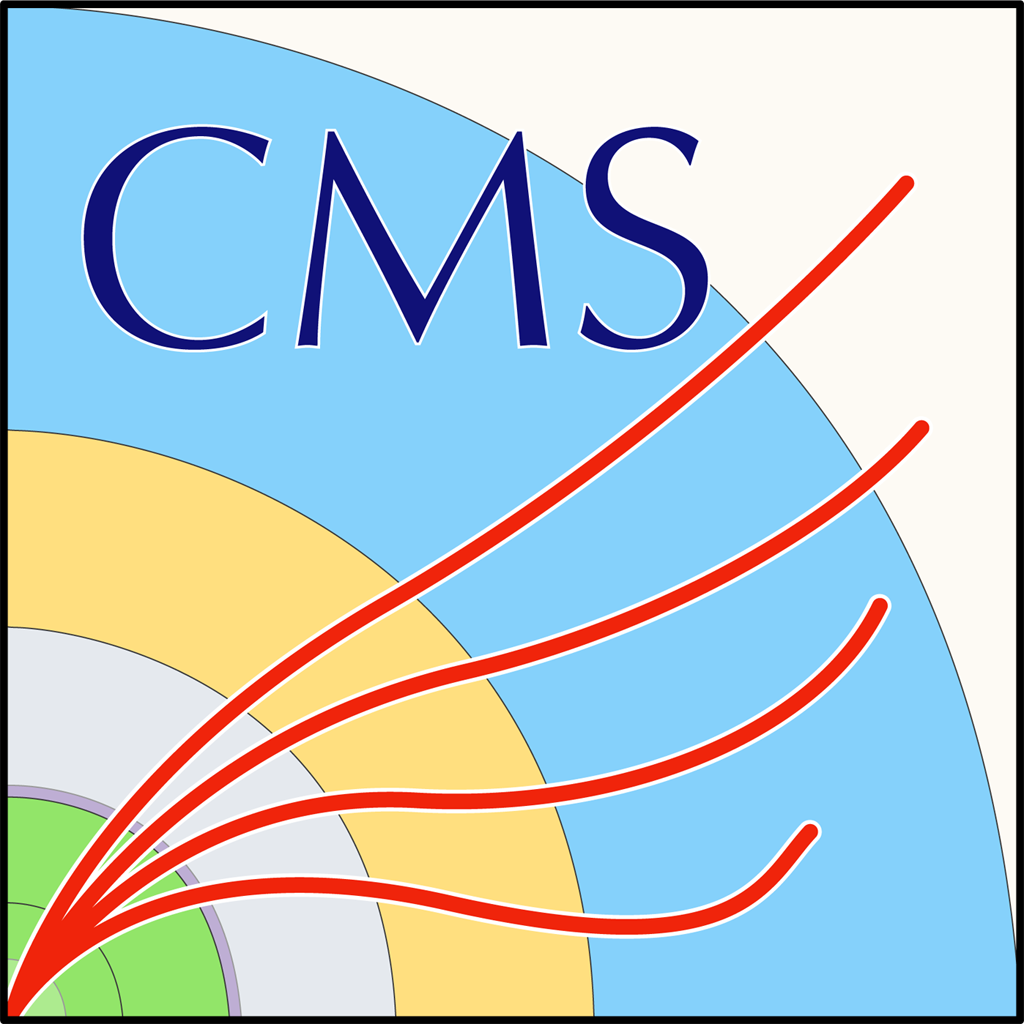
\includegraphics[width=1.5cm]{cms.png}
}

%----------------------------------------------------------------------------------------
%	PRESENTATION SLIDES
%----------------------------------------------------------------------------------------

\begin{document}

\begin{frame}
    % Print the title page as the first slide
    \titlepage
\end{frame}

%\begin{frame}
%	\frametitle{Outline}%
%	\tableofcontents
%\end{frame}

%------------------------------------------------
%\section{Total Cross Sections}
%------------------------------------------------


\begin{frame}{Introduction}
	\begin{columns}[T]
		\begin{column}{.5\textwidth}
			\begin{itemize}
				\item Hadronic cross sections can be decomposed into ...
				\begin{itemize}
					\item Elastic : initial and final states are identical
					\item Diffractive : rapidity gaps, (virtual) meson exchange
					\item Inelastic : hard QCD contribution
				\end{itemize} \vspace{0.15in}	
				\item Precise measurement of hadronic cross section has some importance :
				\begin{itemize}
					\item MC generator tuning parameters as input to phenomenological models
					\item Controlling the PU contribution in pp collision events
				\end{itemize}
			\end{itemize}
		\end{column}
		\begin{column}{.5\textwidth}
			\centering
			\vspace{0.2in}
			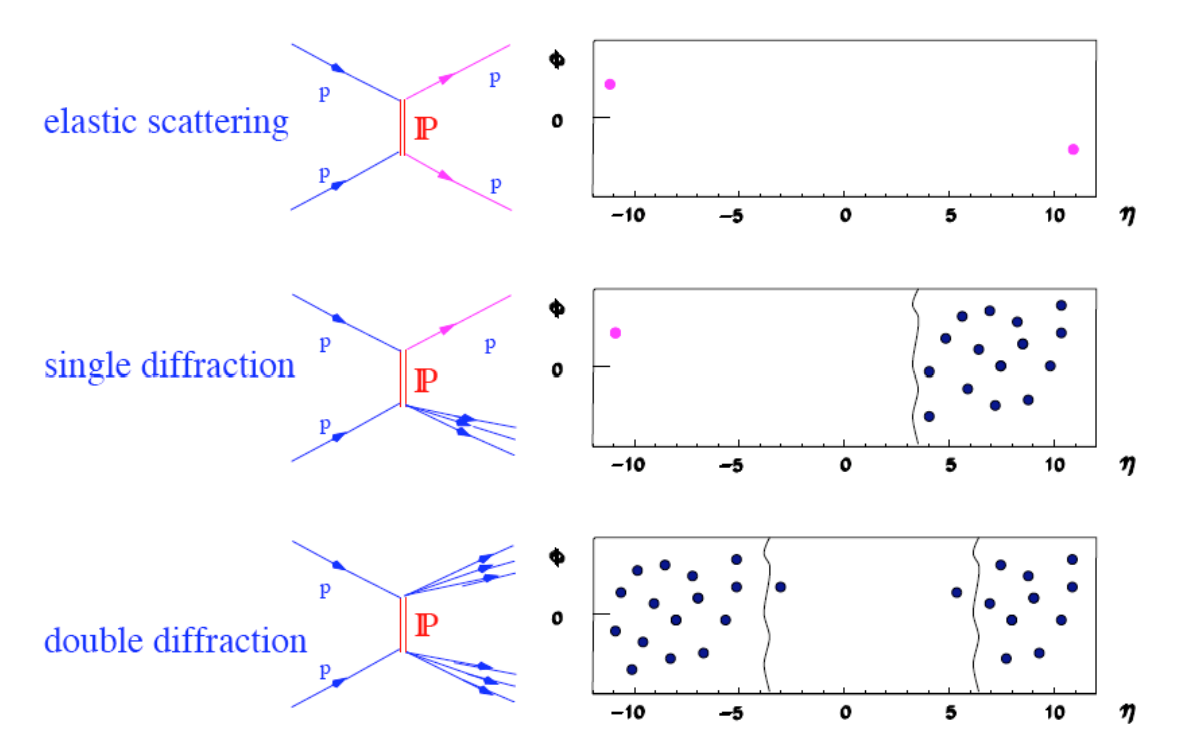
\includegraphics[width=\textwidth]{interactions.png}
		\end{column}
	\end{columns}
\end{frame}



\begin{frame}{Introduction}
	\begin{columns}[T]
		\begin{column}{0.6\textwidth}
				\begin{itemize}
				\item Previous measurements of $\sigma_{inel}$ (mb) :
				\begin{itemize}
					\item CMS (7 TeV) : $ 60.2 \pm 0.2_\text{stat.} \pm 1.1_\text{sys.} \pm 2.4_\text{lum.}  $
					\item TOTEM (8 TeV) : $ 74.7 \pm 1.7 $
					\item ATLAS (13 TeV) : $ 73.1 \pm 0.9_\text{exp.} \pm 6.6_\text{lum.} \pm 3.8_\text{ext.}$
				\end{itemize} \vspace{0.1in}
			\end{itemize}
		\end{column}
		\begin{column}{.4\textwidth}
			\begin{figure}
				\centering
				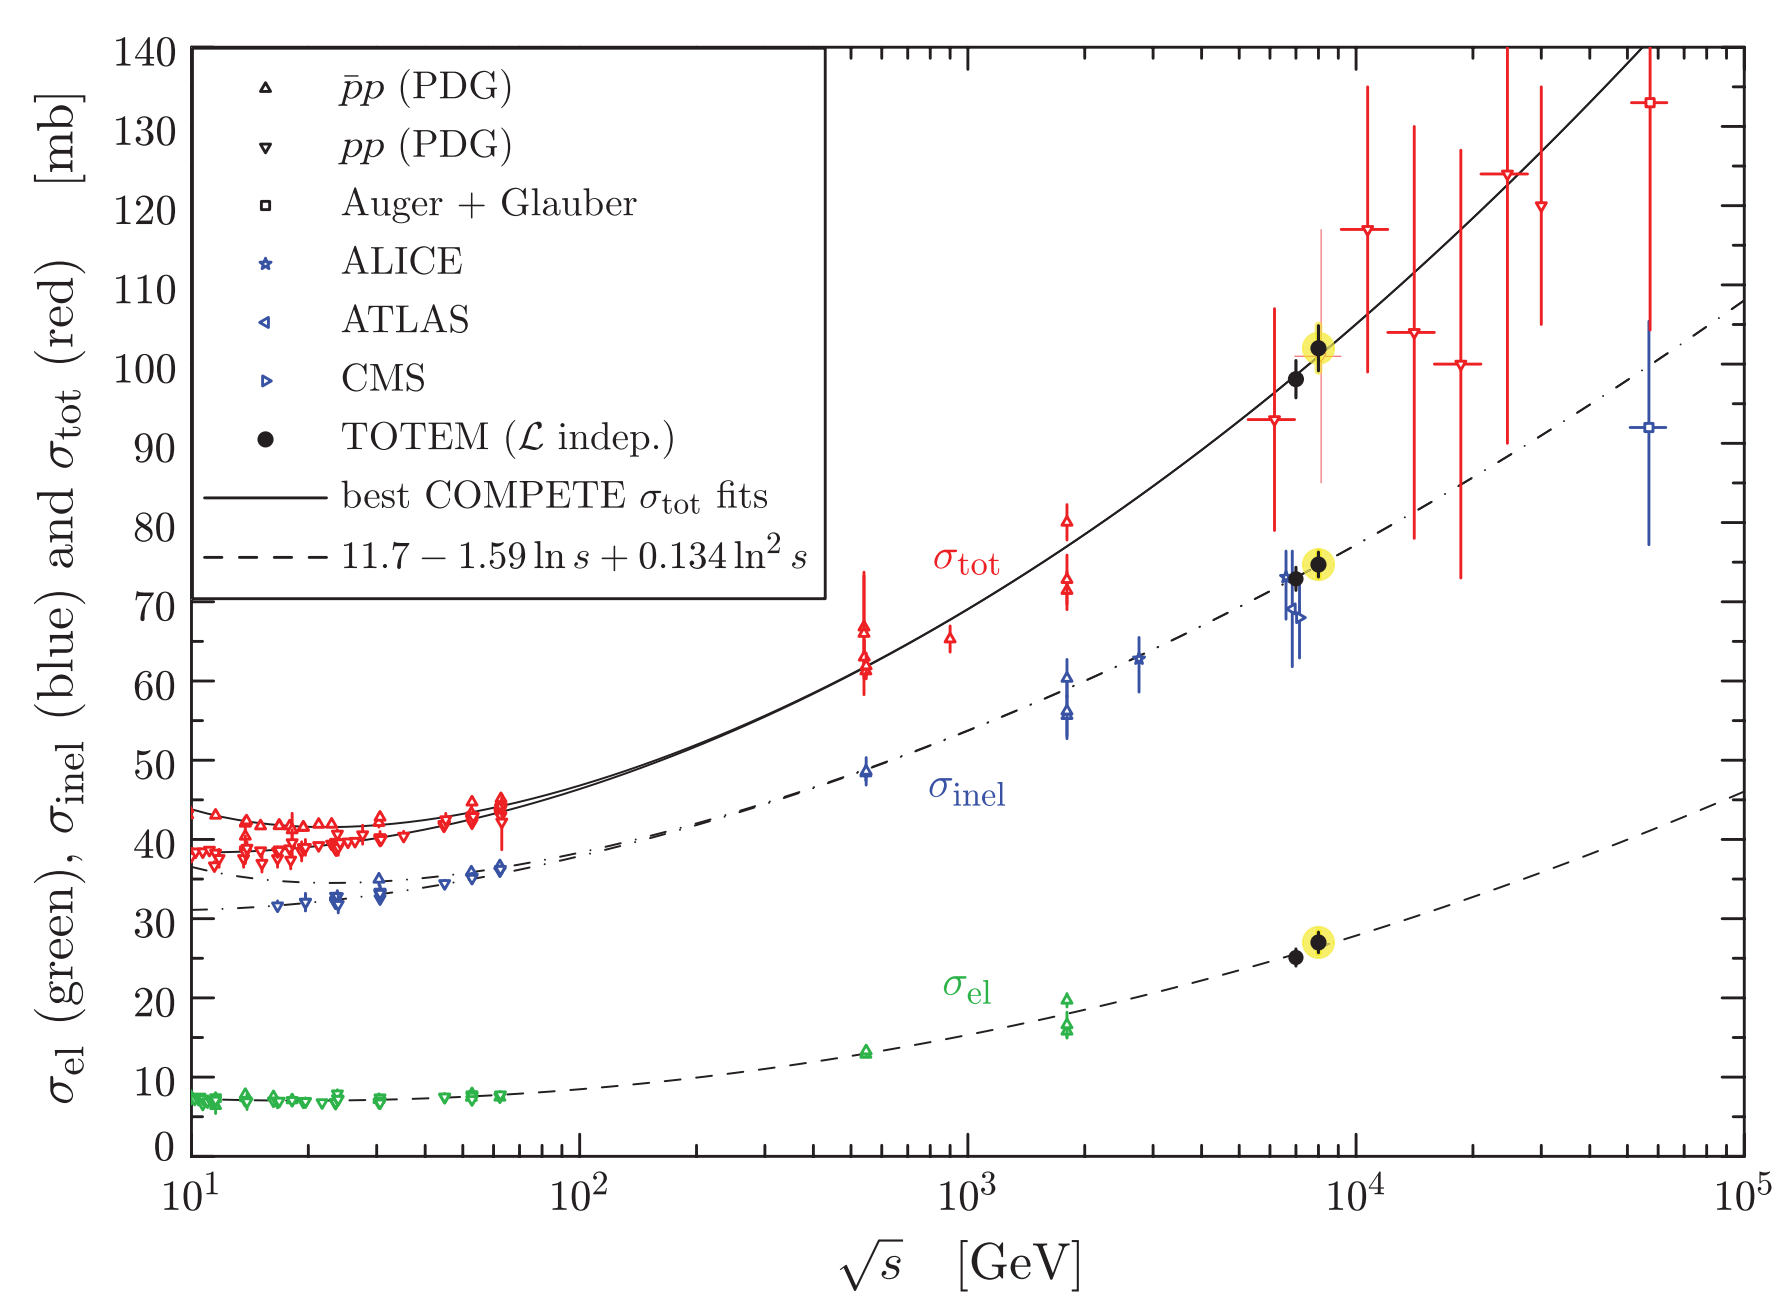
\includegraphics[width=\linewidth]{screenshot004}
 
			\end{figure}
		\end{column}
	\end{columns}

\end{frame}

\begin{frame}{Introduction}
	\begin{columns}[T]
		\begin{column}{0.6\textwidth}
			\begin{itemize}
				\item 13 TeV $\sigma_{inel}$ measurement in CMS :
				\begin{itemize}
					\item Data collected using HFCAL and CASTOR
					\begin{itemize}
						\item Provides sensitivity to a large part of $\sigma_{inel}$ including diffractive ones, leaving particles at forward rapidity
					\end{itemize}
					\item Pseudorapidity region covering :
					\begin{itemize}
						\item $-6.6 < \eta < -3.0$ , $+3.0 < \eta < +5.2$
					\end{itemize}
					\item Phase space region corresponding to :
					\begin{itemize}
						\item $\xi_X > 10^{-7}$ , $\xi_Y > 10^{-6}$
						\item $M_X > 4.1$ GeV , $M_Y > 13$ GeV
					\end{itemize}
				\end{itemize}
			\end{itemize}
		\end{column}
		\begin{column}{.4\textwidth}
			\centering
			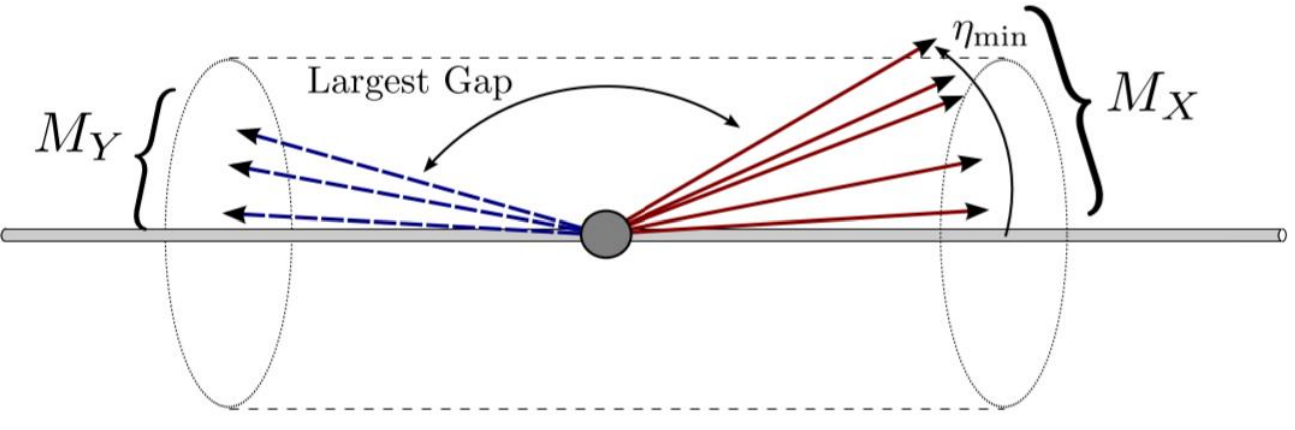
\includegraphics[width=0.85\textwidth]{system.png}
			\vspace{0.1in}
			\begin{align*}
			\xi_X = \frac{M^2_X}{s} &\text{ , } \xi_Y = \frac{M^2_Y}{s} \\
			\xi = \text{max}&(\xi_X , \xi_Y)
			\end{align*}
		\end{column}
	\end{columns}
	
\end{frame}

\begin{frame}{Detectors : Overview}
	\begin{figure}
		\centering
		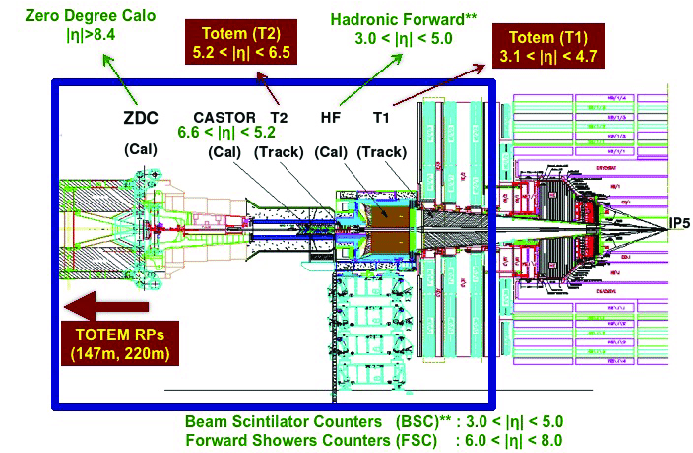
\includegraphics[width=0.7\linewidth]{screenshot001}
	\end{figure}
\end{frame}


\begin{frame}{Detectors : HFCAL}
	\begin{columns}
		\begin{column}{.5\textwidth}
			\begin{figure}
				\centering
				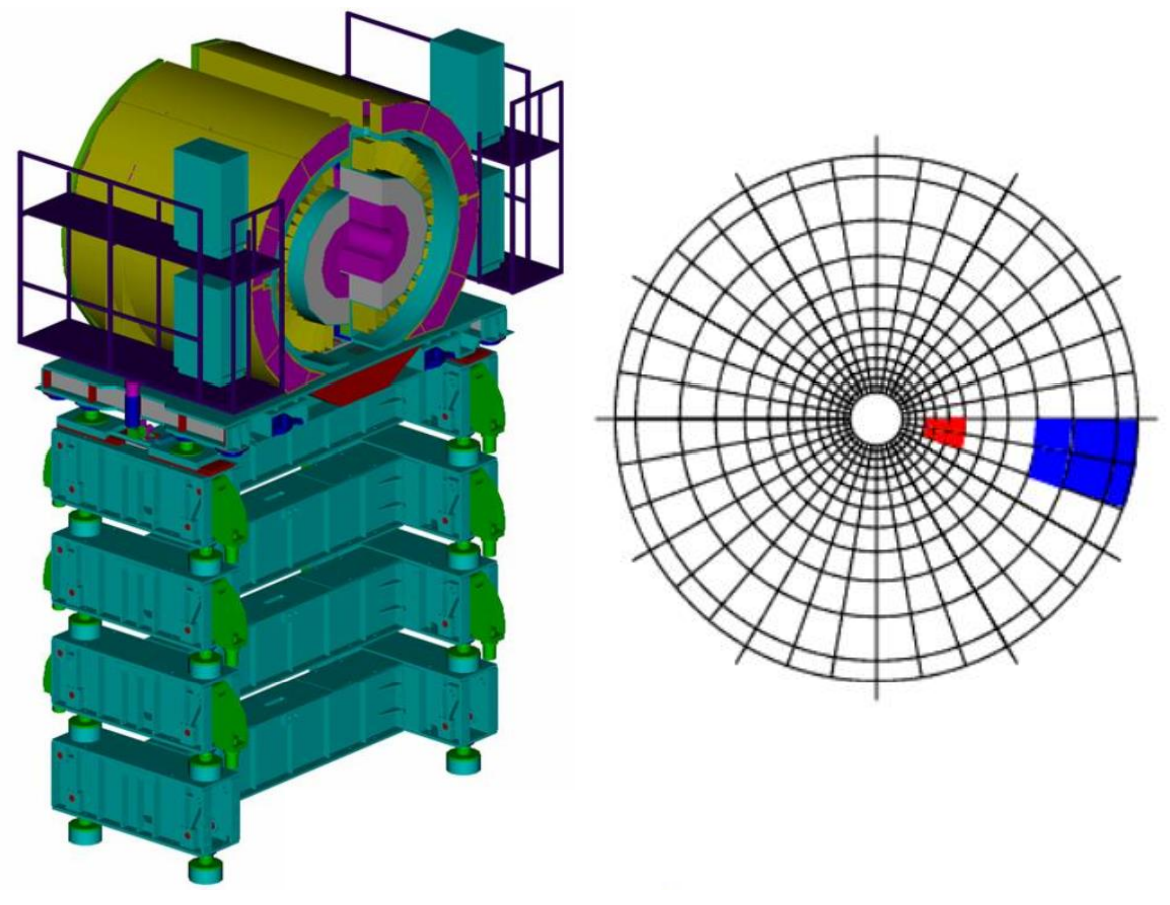
\includegraphics[width=0.8\linewidth]{screenshot002}
			\end{figure}
		\end{column}
		\begin{column}{.5\textwidth}
			\begin{itemize}
				\item HFCAL (\textbf{H}adron \textbf{F}orward \textbf{CAL}orimeter)
				\begin{itemize}
					\item Resides on each side of the detector, covering the region of $3.0 <|\eta|<5.2$
					\item 18 iron azimuthal wedges, embedded with quartz fibers running along the beam direction
					\item Each wedges are subdivided into 13 $\eta$ segments (towers)
				\end{itemize}
			\end{itemize}
		\end{column}
	\end{columns}
\end{frame}

\begin{frame}{Detectors : CASTOR}
	\begin{columns}
		\begin{column}{.35\textwidth}
			\begin{figure}
				\centering
				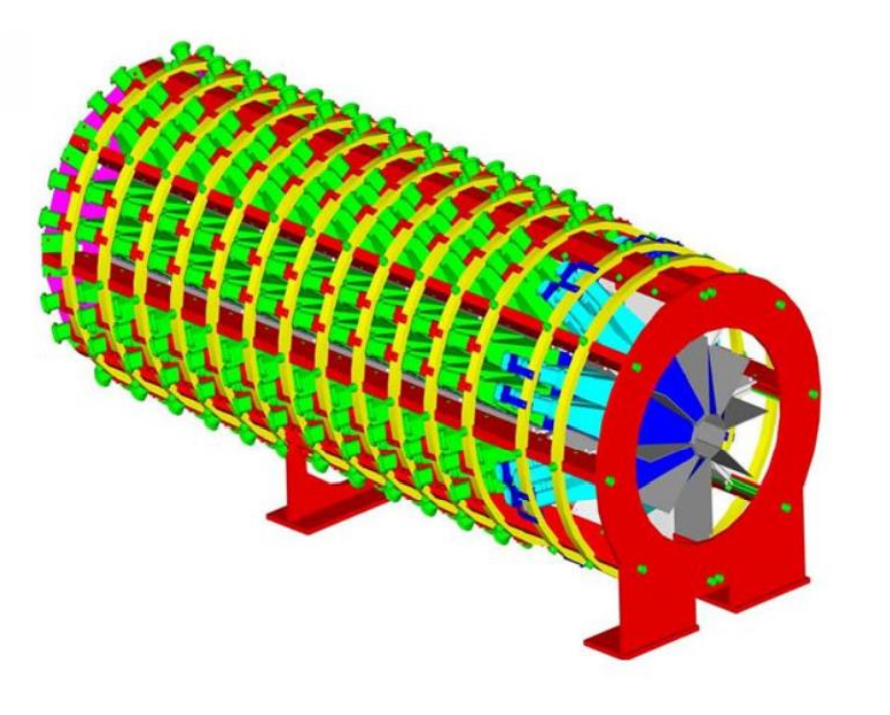
\includegraphics[width=0.7\linewidth]{screenshot003}
			\end{figure}
		\end{column}
		\begin{column}{.65\textwidth}
			\begin{itemize}
				\item CASTOR (\textbf{C}entauro \textbf{A}nd \textbf{ST}range \textbf{O}bject \textbf{R}esearch)
				\begin{itemize}
					\item Installed in one end of the CMS detector, covering the very forward region of $-6.6 < \eta < -5.2$
					\item Tungsten and quartz layers located  $\sim$ 14 m away from IP
					\item 16 $\phi$-sectors and 14 $z$-modules, in total 224 cells.
					\item Was only partially included in the detector setup during the run periods considered on this analysis. 
				\end{itemize}
			\end{itemize}
		\end{column}
	\end{columns}
\end{frame}


\begin{frame}{Event Selection and Reconstruction}
	\begin{itemize}
		\item Based on 2015 pp collision data at $\sqrt{s}=13$ TeV
		\begin{itemize}
			\item $B=0$ T : larger acceptance with CASTOR
			\item $B=3.8$ T (nominal run)
		\end{itemize}
	    \item Integrated luminosity measurement :
	    \begin{itemize}
	    	\item $B=0$ T : obtained using HF or BCM1F detector (12\%)
	    	\item $B=3.8$ T : pixel tracker + Van der Meer scan (2.7\%)
	    \end{itemize}
		\item Triggers used : \texttt{ZeroBias} , \texttt{SingleBunch}, \texttt{EmptyBunch}
		\item Offline Selection
		\begin{itemize}
			\item Requiring an energy deposit $>$ 5 GeV in any of the 2 HF calorimeters. \\ (CASTOR included for $B=0$ T events)
		\end{itemize}
	\end{itemize}
\end{frame}

\begin{frame}{Event Selection and Reconstruction}
	\begin{itemize}
		\item The corrected number of interactions $N_{cor}$ is then obtained : 
		
		\begin{align*}
			N_{cor} = N_{ZB} \left[ (F_{ZB} - F_{EB}) + F_{EB} (F_{ZB} - F_{EB}) \right]
		\end{align*}
		\begin{itemize}
			\item $N_{ZB}$, $N_{EB}$ : number of events triggered by  \texttt{ZeroBias}, \texttt{EmptyBunch}
			\item $F_{ZB}$, $F_{EB}$ : fraction of events selected offline after passing the triggers
		\end{itemize}\vspace{0.1in}
		\item The second term gives a first order correction for signal events overlayed with noise.
	\end{itemize}
\end{frame}

\begin{frame}{Event Selection and Reconstruction}
	\begin{itemize}
		\item The reconstructed number of events is further corrected for the effect of pileup : 
		
		\begin{align*}
		f_{PU} = \frac{\sum_{n=0}^{\infty}nP(n,\lambda)}{\sum_{n=1}^{\infty}P(n,\lambda)} = \frac{\lambda}{1-P(0,\lambda)}
		\end{align*}
		\begin{itemize}
			\item The observed number of pp collisions per bunch crossing $n$, follows a Poisson distribution $P(n,\lambda)$ with the average value $\lambda$
			\item From $P(0,\lambda) = e^{-\lambda}=1-N_{cor}/N_{ZB}$, one could extract $\lambda$ from the data.
		\end{itemize}\vspace{0.1in}
		\item  Then the total reconstructed number of interactions $N_{int}$, is given by
		
		\begin{align*}
			N_{int} = \sum_{\text{bunches}} N_{cor}^b \times f_{PU}^b
		\end{align*} \vspace{0.1in}
		where the corrections are applied bunch by bunch.
	\end{itemize}
\end{frame}

\begin{frame}{Visible $\sigma_{inel}$ Extraction}
	\begin{itemize}
		\item Data are corrected for various detector effects
		\item Detector level selections are chosen to select a sample of inelastic events in the largest possible phase space domain.
		\begin{itemize}
			\item Some low-mass diffractive dissociation might escape the detector acceptance 
			\item Adpating the selected phase space to the detector accpetance results in a smaller correction, leading to smaller model dependence of the correction factors.
		\end{itemize}
	\end{itemize}
	%\begin{figure}
	%	\centering
	%	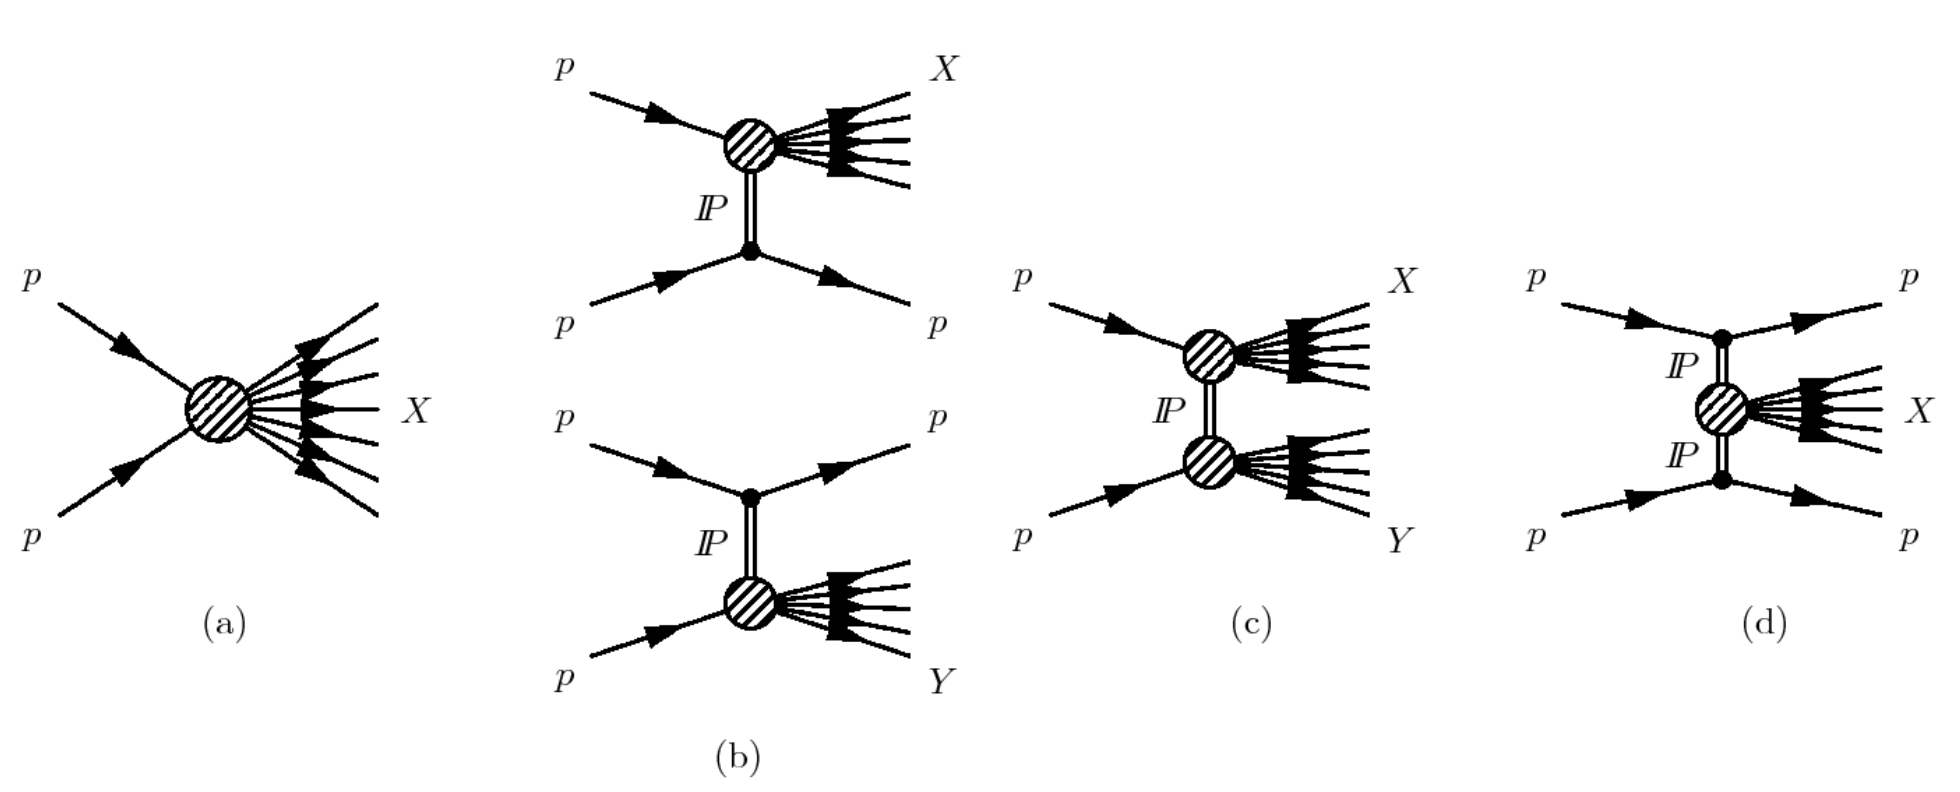
\includegraphics[height=0.25\linewidth]{screenshot005}
	%\end{figure}
\end{frame}

\begin{frame}{Visible $\sigma_{inel}$ Extraction}
	\begin{columns}[T]
	\begin{column}{0.5\textwidth}
		\begin{itemize}
			\item System setup : 
			\begin{itemize}
				\item Collection of stable final-state particles ($c\tau > 1$ cm) with the largest $\eta$ gap is divided into 2 parts $X,Y$
				\item Negative rapidity side is assigned to $X$ (CASTOR side) and vice versa.
			\end{itemize}\vspace{0.1in}
			\item Phase space cut by giving limits on $\xi_{X/Y}$ :
			\begin{itemize}
				\item $\xi > 10^{-6}$ when HF is used alone
				\item $\xi_X > 10^{-7}$ and $\xi_{Y} > 10^{-6}$ when CASTOR is on. (CASTOR lowers the $\xi$ limit)
			\end{itemize}
		\end{itemize}
	\end{column}
	\begin{column}{.5\textwidth}
		\centering
		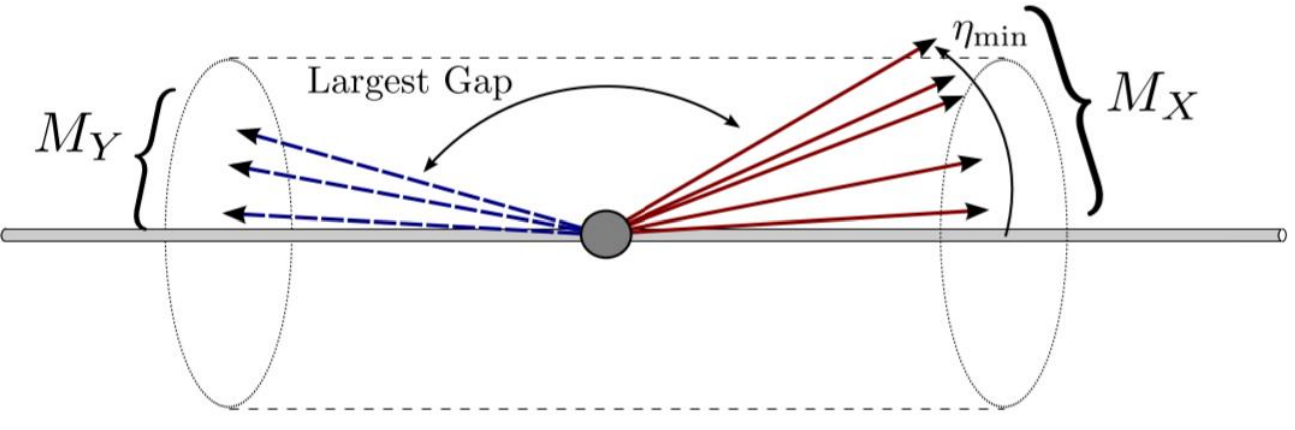
\includegraphics[width=0.85\textwidth]{system.png}
		\vspace{0.1in}
		\begin{align*}
		\xi_X = \frac{M^2_X}{s} &\text{ , } \xi_Y = \frac{M^2_Y}{s} \\
		\xi = \text{max}&(\xi_X , \xi_Y) \\
		\Delta y \sim &\ln(1/\xi)
		\end{align*}
	\end{column}
\end{columns}
\end{frame}

\begin{frame}{Visible $\sigma_{inel}$ Extraction}
	\begin{itemize}
		\item The fully corrected cross section $\sigma$ is calculated as,
		\begin{align*}
			\sigma = \frac{N_{int}(1-b_\xi)}{\epsilon_\xi \int \mathcal{L} dt}
		\end{align*}
		where additional $\epsilon_\xi$ and $b_\xi$ factors are involved. Such factors connect the stable-particle phase space definition and the detector level offline selection. \vspace{0.1in}
		\begin{itemize}
			\item Efficiency  $\epsilon_\xi$ : fraction of selected stable-particle level events that fulfill the detector-level offline selection criteria
			\item Contamination $b_\xi$ : fraction of detector-level offline selected events that are not part of the considered phase space 
		\end{itemize}
	\end{itemize}
\end{frame}

\begin{frame}{Systematic Uncertainties}
	\begin{itemize}
		\item Model Dependence
		\item HF and CASTOR energy scale uncertainty 
		\item CASTOR alignment
		\item Run-to-run variation 
		\item Luminosity 
	\end{itemize}
\end{frame}

\begin{frame}{Systematic Uncertainties}
\begin{figure}
	\centering
	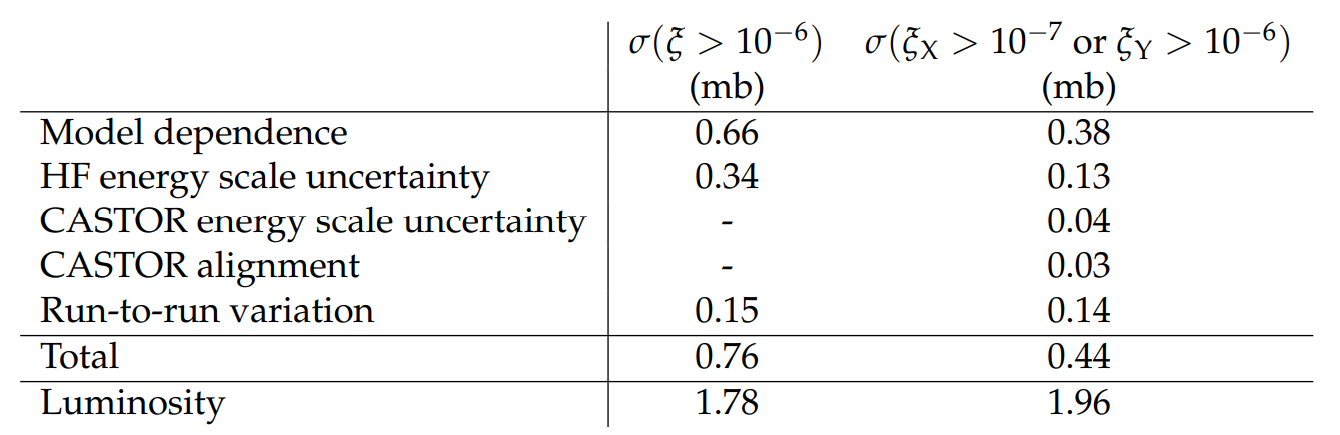
\includegraphics[width=0.85\linewidth]{screenshot006}
\end{figure}

\end{frame}

\begin{frame}{results}
	\begin{figure}
		\centering
		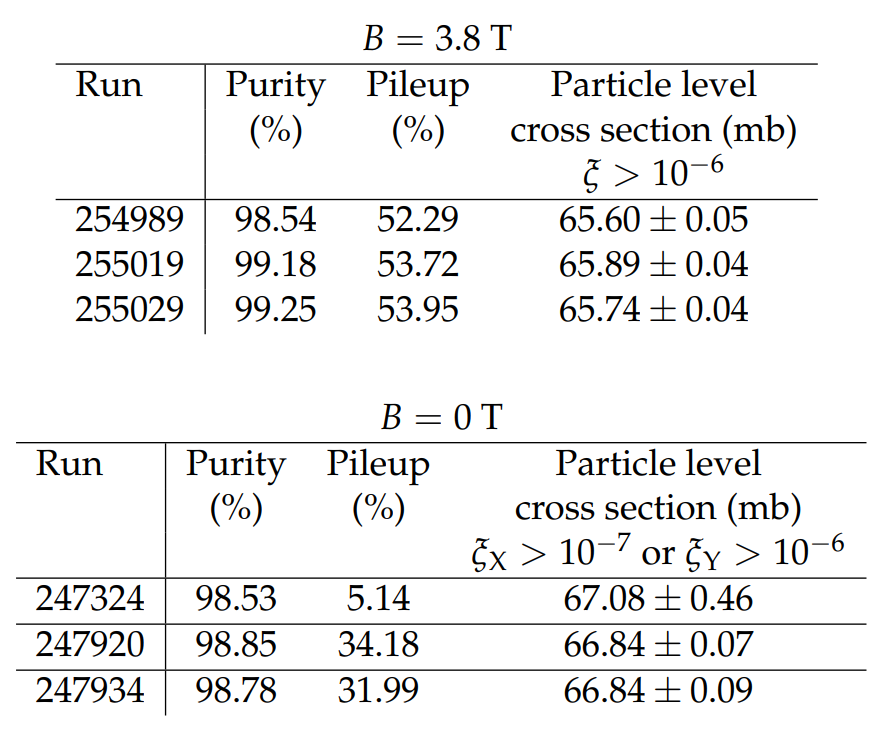
\includegraphics[width=0.5\linewidth]{screenshot009}
	\end{figure}
\end{frame}

\begin{frame}{Results}
	\begin{columns}
		\begin{column}{.5\textwidth}
			\begin{figure}
				\centering
				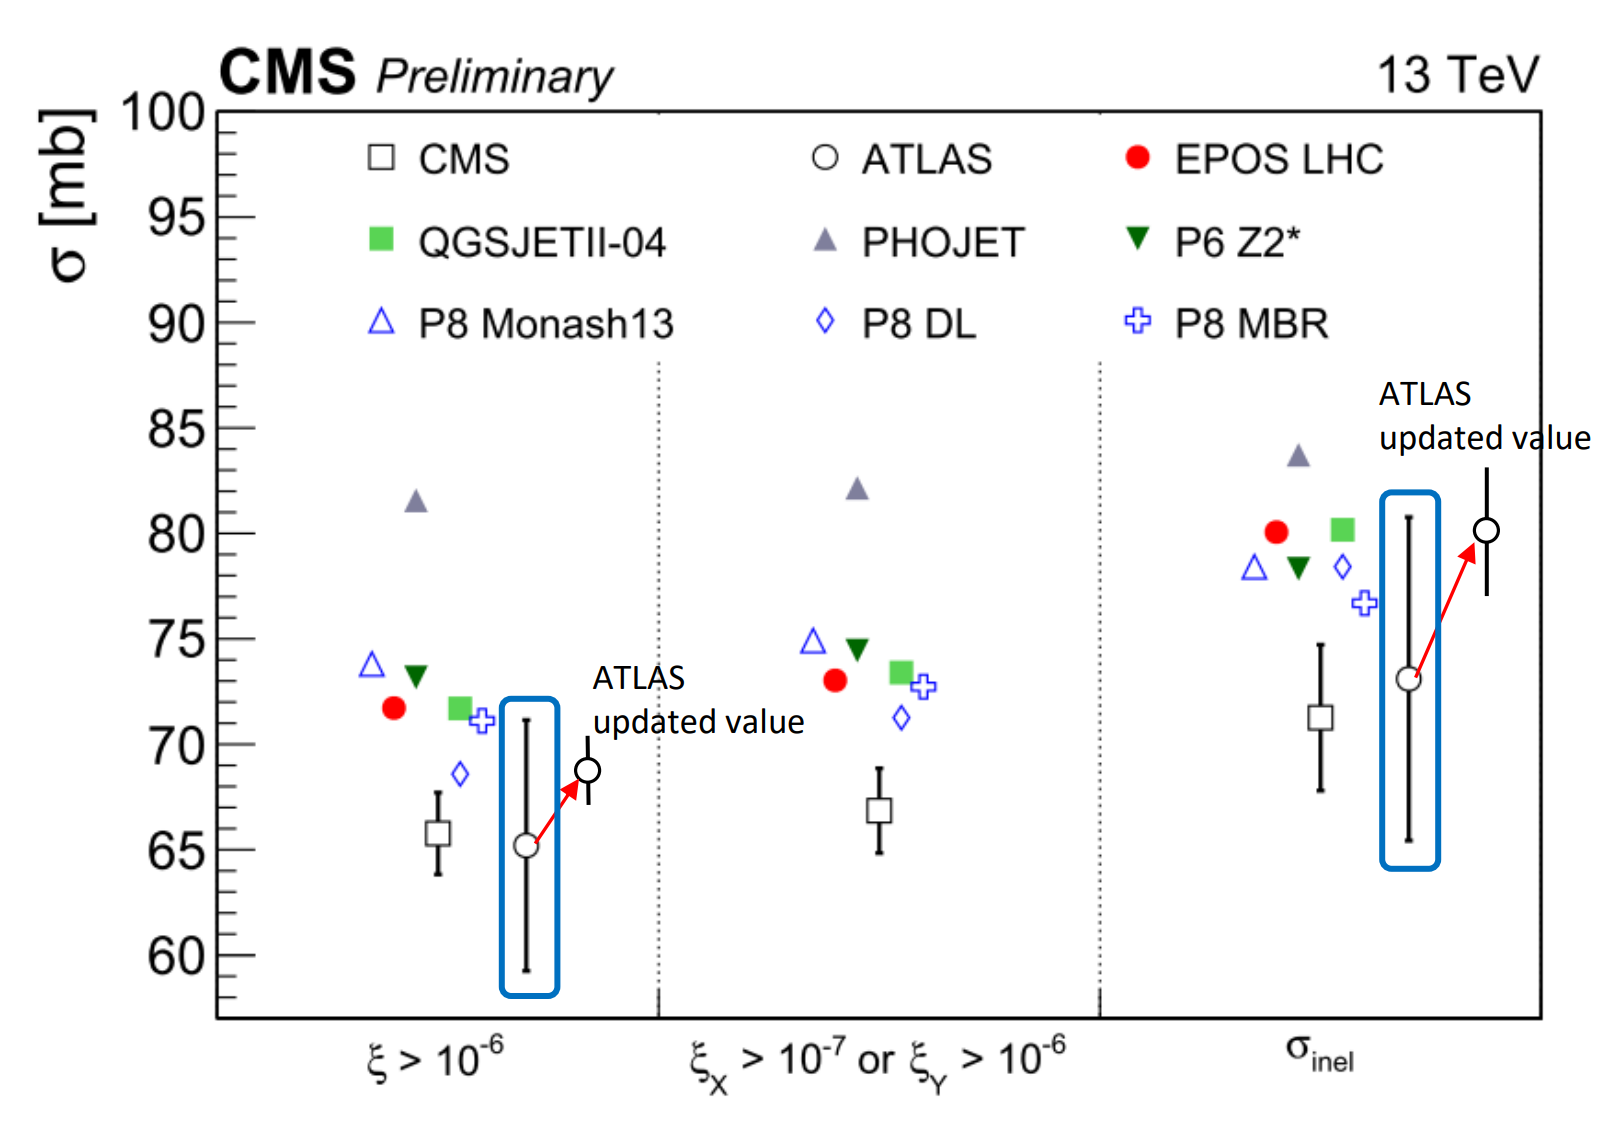
\includegraphics[width=\linewidth]{screenshot007}
			\end{figure}
		\end{column}
		\begin{column}{.5\textwidth}
			\begin{itemize}
				\item For the $B=3.8$ T phase space,\\
				$\sigma(\xi > 10^{-6}) = 65.77 \pm 0.03_\text{stat.} \pm 0.76_\text{sys.} \pm 1.78_\text{lum.} $ mb 
				\vspace{0.1in}
				\item For the extended phase space,\\
				$\sigma(\xi_X > 10^{-7} \text{ or } \xi_Y > 10^{-6} ) = 66.85 \pm 0.06_\text{stat.} \pm 0.44_\text{sys.} \pm 1.96_\text{lum.} $ mb
			\end{itemize}
		\end{column}
	\end{columns}
\end{frame}

\begin{frame}{Results}
	\begin{columns}
	\begin{column}{.5\textwidth}
		\begin{figure}
			\centering
			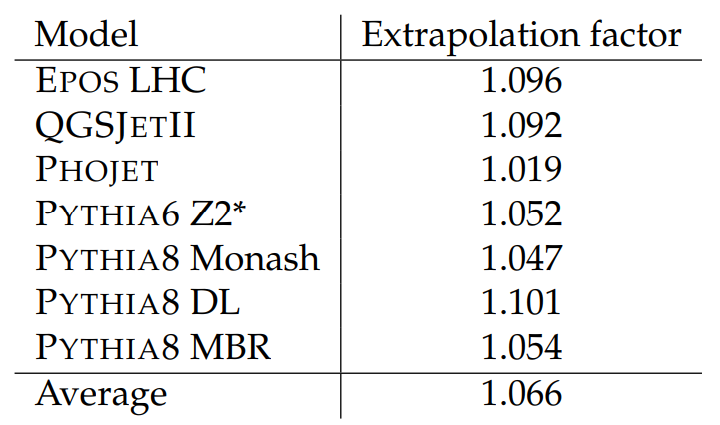
\includegraphics[width=0.8\linewidth]{screenshot008}
		\end{figure}
	\end{column}
	\begin{column}{.5\textwidth}
		\begin{itemize}
			\item Model dependent extrapolation factors are applied, thus giving $\sigma_{inel}$ as, \\[0.15in]
			$\sigma_{inel} = 71.26 \pm 0.06_\text{stat.} \pm 0.47_\text{sys.} \pm 2.09_\text{lum.} \pm 2.72_\text{ext.} $ mb 
			\vspace{0.15in}
			\item Lower than the ATLAS 13 TeV result.
		\end{itemize}
	\end{column}
\end{columns}
\end{frame}

\begin{frame}{Summary}
	\begin{itemize}
		\item A measurement of $\sigma_{inel}$ for pp collisions at $\sqrt{s} = 13 $ TeV with the CMS detector has been presented.
		\item For two phase space regions, visible cross sections were obtained and extrapolated to the total full inelastic phase space domaine, yielding $\sigma_{inel}$ to be 
		\begin{align*}
			\sigma_{inel} = 71.26 \pm 0.06_\text{stat.} \pm 0.47_\text{sys.} \pm 2.09_\text{lum.} \pm 2.72_\text{ext.}  \text{ mb}
		\end{align*}
		\item The measure cross section is significantly lower than predicted by models for hadronic scattering.
	\end{itemize}
\end{frame}

\begin{frame}
    \Huge{\centerline{Thank You}}
\end{frame}

%----------------------------------------------------------------------------------------

\end{document}